\begin{figure}[H]
	\centering
	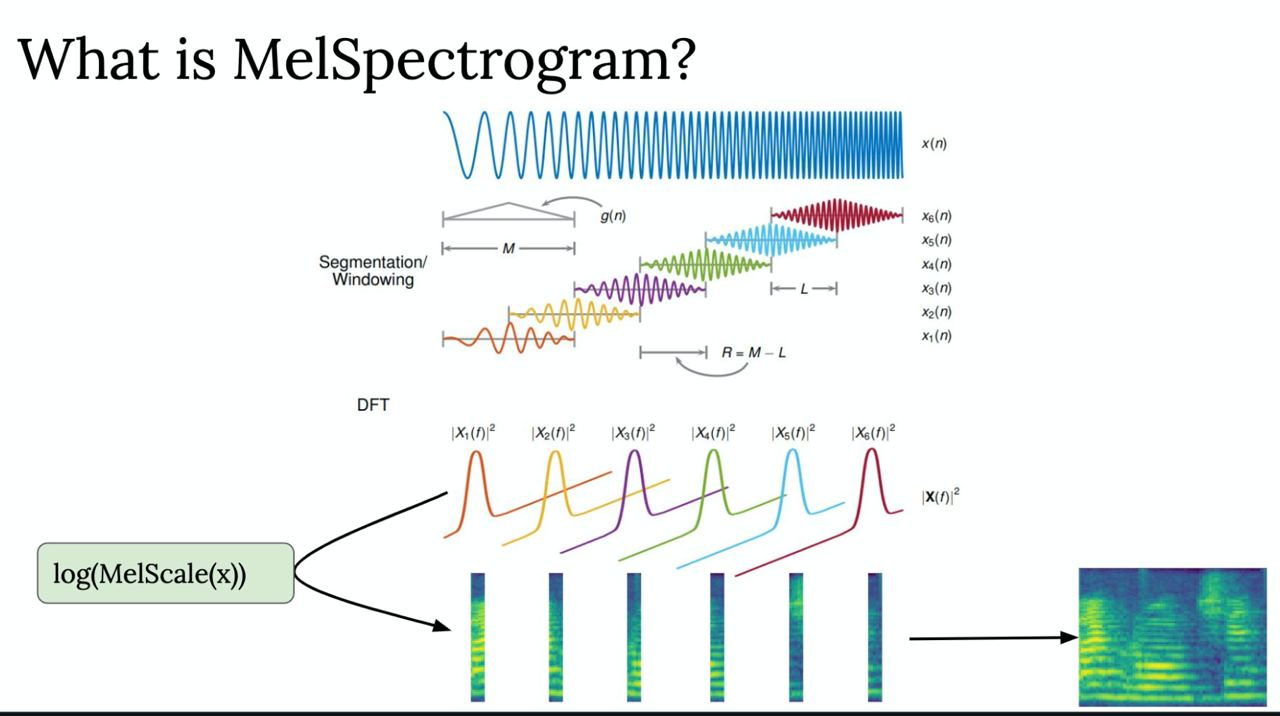
\includegraphics[width=\linewidth]{melspec.jpg}
\end{figure}

Зачем нам вообще спектрограммы? Потому что в одном звуке в сыром сигнале содержится 2000-4000 амплитуд, это дорого хранить. Плюс, мы не инвариантны к шумам и трансформациям. \\

У нас есть исходный сигнал. Мы по нему бежим каким-то окном с каким-то шагом (при этом идем с пересечением -- окна могут накладываться друг на друга). К каждому вырезанному окну мы применяем оконную функцию. Зачем она нужна? На следующем шаге мы будем применять преобразование Фурье, а оно работает с сигналом, который периодичен, то есть он начинается и кончается в нуле (поэтому часто такие фукнции имеют форму 'колокольчика', в домашке например мы применяли косинуисальный фильтр). По сути мы поэлементно перемножаем значение нашего сигнала на значение оконной функции в данной точке. \\ 

Дальше к каждому окошку применяем преобразование Фурье. Суть преобразования Фурье -- представляем сырой сигнал как совокупность синусов и косинусов (например, в форме f(t) = 5 + 2sin(2t + 2) - 3cos(0.2t - 1)). У разных косинусов и синусов будут разные 'веса' и константы. В каждый момент времени каждая отдельная (ко-)синусоида вносит разный вклад в формирование сигнала, веса при них меняются в каждый момент времени. Дискретное преобразование Фурье можно представить как умножение матрицы на окно, которое мы получили на прошлом шаге. Элемент этой матрицы $M_{mn} = exp(-2\Pi i\frac{(m - 1)(n - 1)}{N})$, где N -- длина сигнала. На выходе мы получим вектор той же длины, что исходный, но с мнимыми числами (i.e. от размерности (100,) перешли к размерности (100,2), добавилось второе измерение). \\ 

Далее считаем квадрат комплексной нормы. То есть поэлементно для каждого комплексного числа считаем корень из (квадрат действительной части + квадрат мнимой части). Снова получаем вектор исходного размера (i.e. (100,)). \\ 

Берем первую половину вектора + 1 в силу его симметричности. \\ 

На этом этапе мы получили просто спектрограмму. 
\begin{figure}[H]
	\centering
	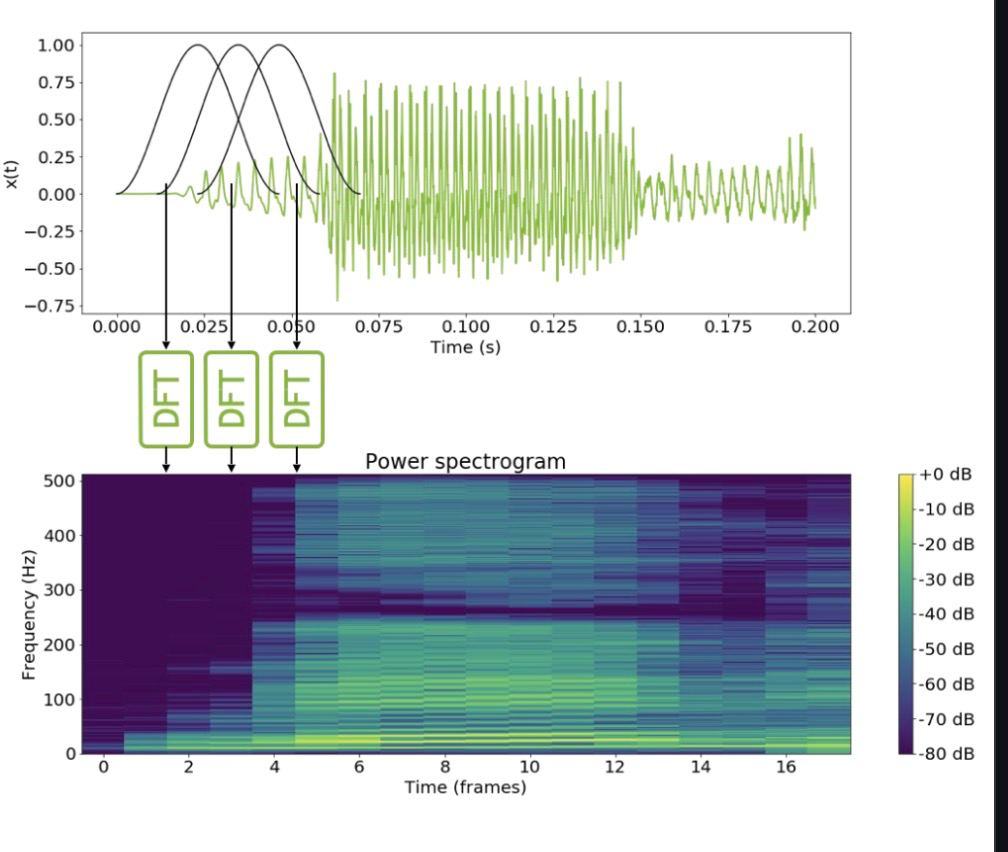
\includegraphics[width=\linewidth]{spec1.jpg}
\end{figure}

Один фрейм (столбик) в спектрограмме -- один раз мы выполнили всю операцию выше. Чем выше идем по столбику, тем более высокие частоты кодируются. Яркость цвета -- насколько в этот момент звучала та или иная частота. Желтый внизу -- это были басы, желтый вверху -- это был писк. \\ 

Как теперь перейти к мелспректрограмме? Для каждого фрейма мы храним все 500 значений частот, хотя часто там наблюдается пустота. Плюс, люди хорошо слышат низкие частоты, а высокие не очень различают. Поэтому мы хотим учесть низкие частоты больше, а высокие -- меньше. Для этого переводим все в мел-шкалу (также реализуемо матричным умножениям). m = 2595$log_{10}(1 + \frac{f}{700})$, где f -- значение частоты, а m -- уже значение мелчастоты. Потом еще берем логарифм от мелспектрограммы. \\ 

Эта шкала лучше отражает, что человеческое ухо слышит. Проблема одна -- это преобразование идет не через квадратную матрицу, поэтому восстановить оригинальный сигнал уже не получится. 
